\chapter{Fitting Star Formation Laws Using Hierarchical Bayesian Regression}
\pagestyle{plain}
\label{app:bays_fitting}
\myappendices

In Chapter~\ref{ch: paper1}, we mentioned that we used hierarchical Bayesian linear regression to fit the star formation laws (both the Kennicutt-Schmidt and the extended Schmidt law).
The goal is to find the star formation laws using observational data.
In order to compare our results with previous studies and testing star formation laws, we chose to use linear regression to fit the data.
Hierarchical Bayesian regression fitting method were chosen over the simple linear regions methods (e.g. ordinary least square fitting) due to fact that this method thoroughly accounts for all the measured uncertainties and considers the hierarchical data structure (if there is any).
\cite{Shetty13} described the fitting using hierarchical Bayesian linear regression in detail.
In this section, we first summarize \cite{Shetty13} approach and show the differences between ordinary least square fitting and the hierarchical Bayesian linear regression and then we describe how we extended their code to fit multiple hierarchical Bayesian regression in order to investigate the extended Schmidt law.

\cite{Shetty13} assumed Bayes' theorem:
\begin{equation}
  \mathcal{P}({\Theta | \mathcal{D}})  \propto \mathcal{P}({\mathcal{D}|\Theta})\mathcal{P}(\Theta)
\end{equation}
where $\Theta$ is the model parameters and $D$ is the data.
$\mathcal{P}({\Theta | \mathcal{D}})$, which is called posterior, is the result of the Bayesian interface.
Posterior is the probability distribution of the model parameters given data. 
$\mathcal{P}(\Theta)$ is the prior on $\Theta$, and $\Theta$ is a vector of all the parameters that define the model.
In the case of the Kennicutt-Schmidt law, $\Theta$ contains power-law index (which is in the log-log basis is the slop,  {\it N}) and intercept, A, (from Equation~\ref{eq:sfr_law_ks_log}), their mean values and variance for each pixel. 
$\mathcal{P}({\mathcal{D}|\Theta})$ is the probability of the data given model parameter, also known as the likelihood.


Given the measured values of the \sigmagas and \sigmasfr and their uncertainty, the Bayesian analysis performs Markov Chain Monte Carlo simulations (MCMC) to find the true value of \sigmagas and \sigmasfr.
The posterior is a probability distribution function for each parameter of $\Theta$ is the the output of the analysis after a large number of MCMC steps (here we chose 50000 steps).

\begin{figure}
\centering
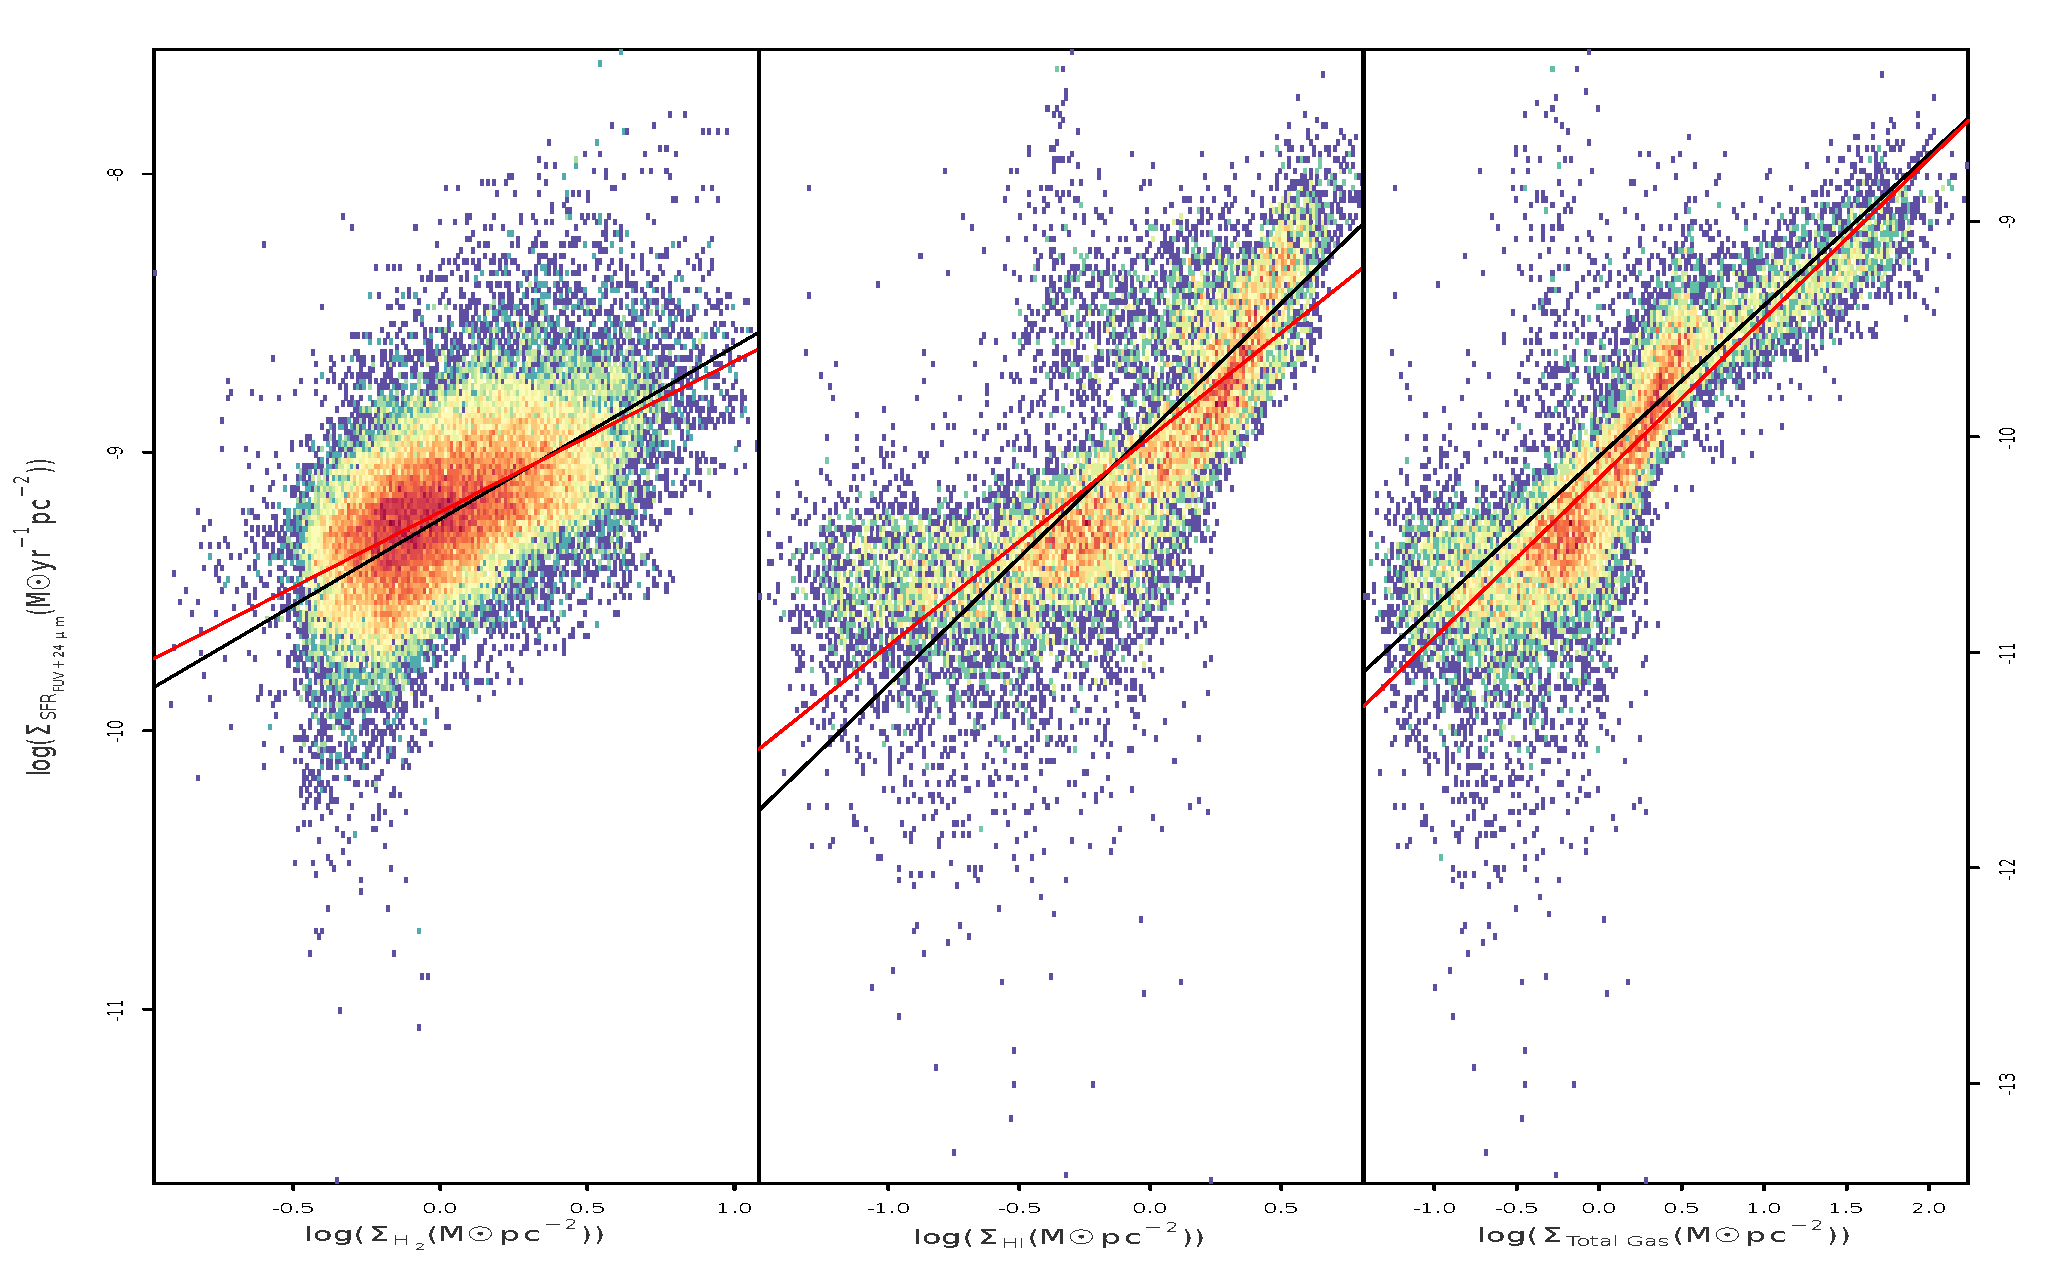
\includegraphics[width=164mm]{../image_paper1/OLS_vs_bayes.png.pdf}
\caption[]{Mosaic created using the Montage programme from six fields of \halpha\ emission images of M31 from \citet{Massey07}. The resulting image from Montage was continuum-subtracted and masked for all point sources. The centre of the galaxy was masked out due to saturation of data in the continuum $R$-band image.}
\label{fig:halpha}
\end{figure}

For finding probability distribution function of parameters of the extended Schmidt law, we followed the similar procedure as \cite{Shetty13}.
Since in the extended Schmidt law, the \sigmasfr depends on two independent variables (\sigmagas and \sigmastar), we used the multiple hierarchical Bayesian linear regression instead on the hierarchical Bayesian linear regression.
We assumed $\Theta$ contains $\eqnprime$, $\beta$, A$^\prime$ from Equation~\ref{eq:sfr_law_es_log}, their mean values and their uncertainties. 
As a result of the analysis we have a distributions of plausible values for the parameters of the star formation laws, which are measured by considering the measured values of the \sigmagas, \sigmasfr, \sigmastar and their uncertainties for each pixel.


\bibliographystyle{apj.bst}
\bibliography{ref_paper1.bib}